\documentclass{article}
\usepackage{amsmath, amsthm} 
\usepackage{enumerate} 
\usepackage[utf8]{inputenc}
\usepackage{polski}
\usepackage{lmodern,microtype}
\usepackage{multicol}
\usepackage{listings}
\usepackage{graphicx}
\usepackage{verbatim}
\usepackage{color}

\author{Matylda Mordal}
\title{\textbf{Tytuł}}
\date{}

\theoremstyle{definition}
\newtheorem{definition}{Definicja}
\newtheorem{theorem}{Twierdzenie}
\newtheorem{corollary}{Wniosek}

\lstset{
	language=Python,         
	basicstyle=\ttfamily,    
	keywordstyle=\color{blue},
	commentstyle=\color{green}, 
	stringstyle=\color{red},    
	numbers=left,           
	numberstyle=\small,     
	stepnumber=1,           
	showstringspaces=false,
	tabsize=4               
}


\begin{document}

	\maketitle
	\section{Sekcja Numerowana}
	Jakiś tekst
	\subsection{Podsekcja Numerowana}
	Jakiś tekst
	
	\section*{Sekcja Nienumerowana}
	Jakiś tekst
	\subsubsection*{Podsekcja Nienumerowana}
	Jakiś tekst
	
	\begin{definition}
	To jest przykładowa definicja.
	\end{definition}
	
	\begin{theorem}
	To jest przykładowe twierdzenie.
	\end{theorem}
	
	\begin{proof}
	Jakiś dowód.
	\[
	a^2 + b^2 = c^2
	\]
	\end{proof}
	
	\begin{corollary}
	Jakiś wniosek
	\end{corollary}
	
	\begin{enumerate}[a)]
		\item To jest wyliczenie numerowane.
		\item Kolejny element wyliczenia numerowanego.
	\end{enumerate}
	
	\begin{itemize}
		\item To jest wyliczenie nienumerowane.
		\item Kolejny element wyliczenia nienumerowanego.
	\end{itemize}
	
	\begin{enumerate}
		\item To jest wyliczenie numerowane.
		\item Kolejny element wyliczenia numerowanego.
	\end{enumerate}
	
	
	\begin{lstlisting}
		#Przykladowy kod w Pythonie
		def mnozenie(x,y):
			return x*y
		print(mnozenie(2,3))
	\end{lstlisting}
	
	\begin{figure}
		\centering
		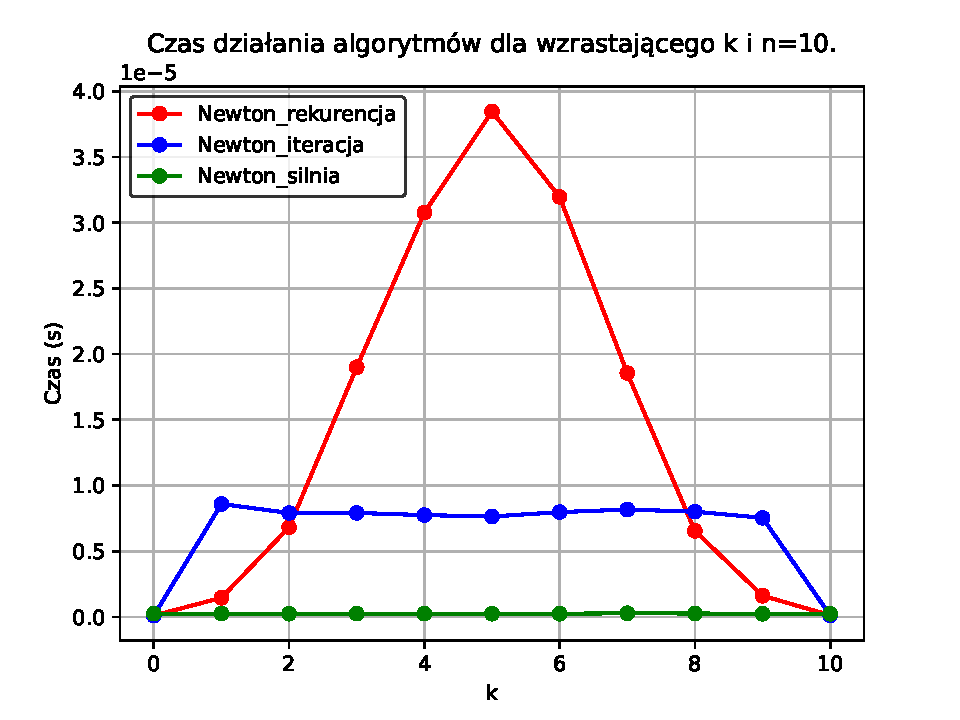
\includegraphics[width=0.9\textwidth]{Wykres2_1.pdf}
	\end{figure}
	
	\begin{verbatim}
		Jakiś tam tekst
	\end{verbatim}
	
	\begin{table}
		\centering
		\begin{tabular}{|c|c|c|}
			\hline
			Kolumna 1 & Kolumna 2 & Kolumna 3 \\ \hline
			Wiersz 1  & Dane 1    & Dane 2    \\ \hline
			Wiersz 2  & Dane 3    & Dane 4    \\ \hline
		\end{tabular}
		\caption{Jakaś tabela}
	\end{table}
	
	\section{Tryb matematyczny}
	Jakiś tekst $a=15$.\\
	Wstawiamy równania w trybie matematycznym:
	\[
	E = mc^2
	\]
	
	Możemy również wstawić równanie numerowane:
	\begin{equation}\label{całka}
		\int_a^b f(x) \, dx = F(b) - F(a)
	\end{equation}
	
	równanie \eqref{całka} na stronie \pageref{całka}
	
	\section{Bibliografia}
	Przykład bibliografii w formacie \texttt{thebibliography}:
	
	\begin{thebibliography}{9}
		
		\bibitem{latexcompanion} 
		Leslie Lamport. 
		\textit{LaTeX: A Document Preparation System}. 
		Addison Wesley, 1986.
		
		\bibitem{einstein} 
		Albert Einstein. 
		\textit{Zur Elektrodynamik bewegter Körper}. (German) 
		\textit{Annalen der Physik}, 1905.
		
	\end{thebibliography}
	
	
\end{document}